%pdflatex --shell-escape --synctex=1 Diapo.tex

\documentclass[11pt, sans,xcolor=table]{beamer}
\usepackage[utf8]{inputenc}
\usepackage{default}
\usepackage{amssymb}
\usepackage{graphicx}
\usetheme{Warsaw}

\title{Développement d'un jeu de type Bomberman en réseau sous Android et iOS}
\author{KLOB}
\institute{Université Montpellier II}
\subtitle{TER}

\begin{document}

\begin{frame}
\titlepage
\end{frame}


\begin{frame}{Sommaire}
\setcounter{tocdepth}{1}
\tableofcontents
\end{frame}

\section{Introduction}

\begin{frame}
\frametitle{Introduction}

	\begin{center} 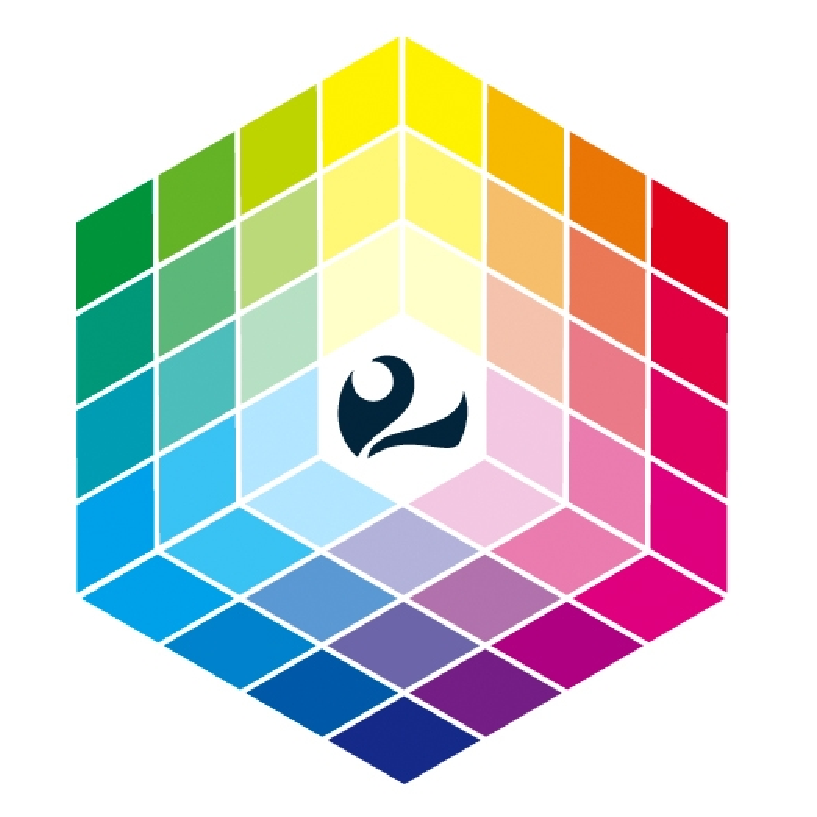
\includegraphics[scale=0.4]{img/logoUm2.eps} \end{center}

\end{frame}



\section{Présentation}

\subsection{Les jeux sur smartphone}

\begin{frame}
\frametitle{Présentation}
\framesubtitle{Les jeux sur smartphone}
Le marché des jeux vidéos sur console portable connait une réel expansion: \\ 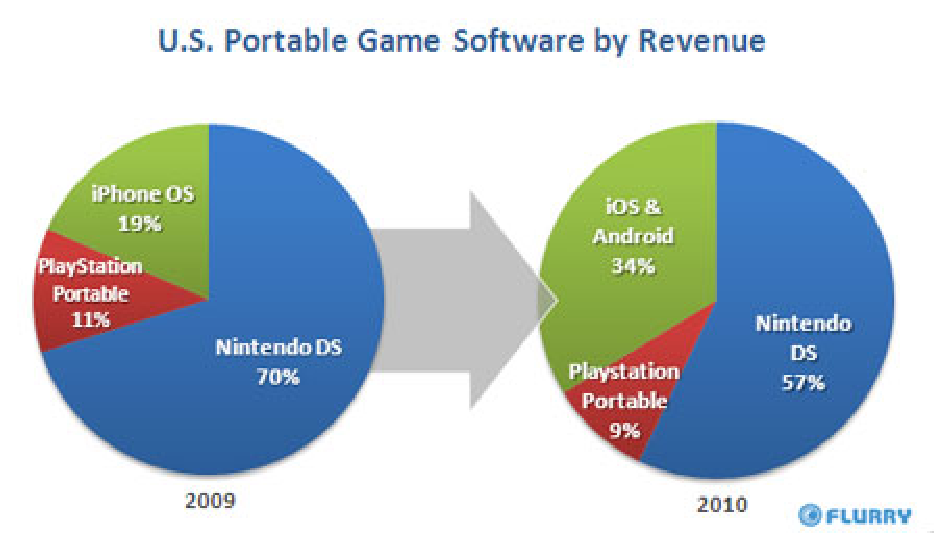
\includegraphics[scale=0.4]{img/marche_console_portable.eps} 

\begin{itemize} 
		\item{Coût peu couteux.}
		\item{Grand nombre de mini-jeux et de jeux.}
		\item{Public visé plus large.}
\end{itemize}
\end{frame}



%%%%%%%%%%%%%%%%%%%%%%%%%%%%%%%%%%%%%%%%%%%%
\subsection{Les sytèmes d'exploitations}


\begin{frame}
\frametitle{Présentation}
\framesubtitle{Android}

	\begin{minipage}{8cm}
		Le système d'exploitation possède : \\ 

	\begin{itemize} 
		\item Noyaux linux pour exploiter le matériel
		\item Librairies connues et open source (OpenGL ES, SQLite,...)
		\item Machine virtuelle Java (Dalvik virtual machine)
		\item API Java riche (package de Java SE, open source ou spécifique au système)
	\end{itemize}
	\end{minipage} & 
\includegraphics[scale=0.2]{img/android.eps} 

\end{frame}


%%%%%%%%%%%%%%%%%%%%%%%%%%%%%%%%%%%%%%%%%%%%


\begin{frame}
\frametitle{Présentation}
\framesubtitle{Android}
	\begin{minipage}{8cm}
	Les possibilités de développement sont: \\ 

	\begin{itemize}
		\item Langage principale Java, développement en C/C++ possible
		\item Kit de développement multiplateforme
		\item Développement sur téléphone ou sur émulateur
		\item Déploiement des applications peu coûteux
	\end{itemize}
	\end{minipage} & 
\includegraphics[scale=0.2]{img/android.eps} 
\end{frame}


%%%%%%%%%%%%%%%%%%%%%%%%%%%%%%%%%%%%%%%%%%%%


\begin{frame}
\frametitle{Présentation}
\framesubtitle{iOS}
	\begin{minipage}{8cm}
Le système d'exploitation possède : \\

	\begin{itemize} 
		\item Noyau hybride XNU dérivé de Mac OS X
		\item Librairies connues et open source (OpenGL ES, SQLite,...)
		\item Pas de machine virtuelle. Code compilé en C.
		\item API Objective-C riche (Core OS, Cocoa Touch,...)
	\end{itemize}
	\end{minipage} & 
\includegraphics[scale=0.2]{img/apple.eps} 
\end{frame}


%%%%%%%%%%%%%%%%%%%%%%%%%%%%%%%%%%%%%%%%%%%%


\begin{frame}
\frametitle{Présentation}
\framesubtitle{iOS}
	\begin{minipage}{8cm}
	Les possibilités de développement sont: \\ 

	\begin{itemize}
		\item Langage principale Objective-C, développement en C possible
		\item Kit de développement disponilbe sur Mac OS seulement
		\item Développement sur téléphone ou sur émulateur (nécessite un compte payant pour tester sur téléphone)
		\item Déploiement des applications coûteux
	\end{itemize}
	\end{minipage} & 
\includegraphics[scale=0.2]{img/apple.eps} 
\end{frame}


%%%%%%%%%%%%%%%%%%%%%%%%%%%%%%%%%%%%%%%%%%%%
\subsection{Le jeu Bomberman}


\begin{frame}
\frametitle{Présentation}
\framesubtitle{Le Bomberman}
\begin{minipage}{7cm}
Histoire
	\begin{itemize}
		\item Jeu d'action.
		\item Première sortie en 1987.
		\item Développé sur plusieurs consoles.
		\item Succès grâce au mode multijoueur sur certaines consoles.
	\end{itemize} \\
\end{minipage} & 
\includegraphics[scale=0.3]{img/bomberman1.eps} 

\end{frame}


%%%%%%%%%%%%%%%%%%%%%%%%%%%%%%%%%%%%%%%%%%%%


\begin{frame}
\frametitle{Présentation}
\framesubtitle{Le Bomberman}
Principe : \\ \\

\begin{minipage}{5cm}
	\begin{itemize}
		\item Le joueur incarne un poseur de bombes.
		\item But du jeu: détruire ses ennemis.
	\end{itemize} \\
\end{minipage} &  \begin{minipage}{5.5cm}
	\begin{itemize}
		\item Multiple bonus (Bonus de vie, de bombes, de vitesse,...).
		\item Multiple malus (Obligation de poser des bombes,...).
	\end{itemize} \\
\end{minipage} 

\begin{center} 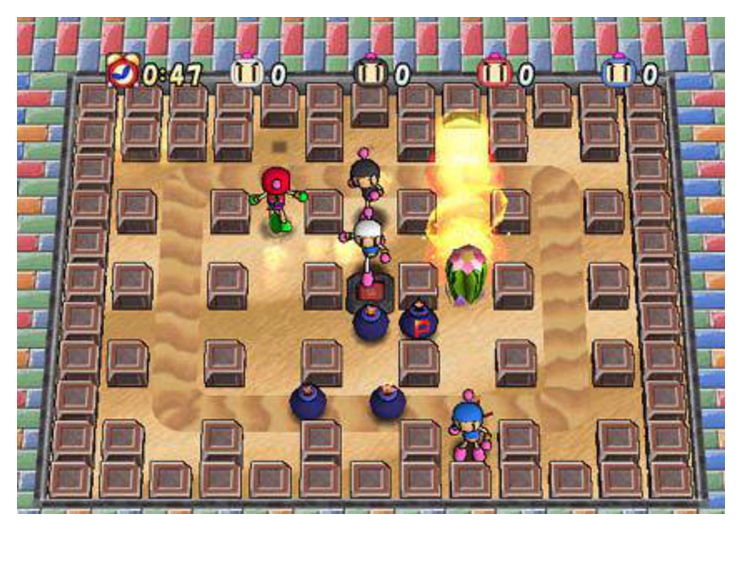
\includegraphics[scale=0.35]{img/bomberman2.eps} \end{center}

\end{frame}


%%%%%%%%%%%%%%%%%%%%%%%%%%%%%%%%%%%%%%%%%%%%
\subsection{Rapport avec l'enseignement}


\begin{frame}
\frametitle{Présentation}
\framesubtitle{Rapport avec l'enseignement}
Ce TER nous a permis de mettre en application les connaissances acquises dans nos parcours d'enseignements  pour: \\

	\begin{itemize}
		\item L'intelligence artificielle (parcours I2A).
		\item Les communications avec le serveur (parcours CASAR).
		\item L'utilisation de servlet (parcours DIWEB).
	\end{itemize} \\
	
\end{frame}





\include{application1}

\section{Discussion}

	\subsection{Difficultés}
		\begin{frame}
			\frametitle{Discussion}
			\framesubtitle{Difficultés}
				\begin{tabular}{cc}
					Android & iOS \\
					\begin{minipage}{5cm}
						\begin{itemize}
							\item Nouvelle plate-forme
							\item Multi-touch
							\item Ressources limitées
						\end{itemize}
					\end{minipage}
					&
					\begin{minipage}{5cm}
					\begin{itemize}
						\item Nouveau langage (Objective-C)
						\item Nouvelle plate-forme
						\item Gestion manuelle de la mémoire
						\item Ressources limitées
					\end{itemize}
				\end{minipage}
			\end{tabular}
		\end{frame}
		
		
	\subsection{Problèmes}
		\begin{frame}
			\frametitle{Discussion}
			\framesubtitle{Problèmes}
			Android et iOS :
			\begin{itemize}
				\item Tester l'application
				\item OpenGL ES
			\end{itemize}
		\end{frame}
		
		
	\subsection{Améliorations}
		\begin{frame}
			\frametitle{Discussion}
			\framesubtitle{Améliorations}
			\begin{itemize}
				\item Mode histoire
				\item Ajout de bonus / malus
				\item Rajout de types de parties
			\end{itemize}
		\end{frame}


\section{Conclusion}

\begin{frame}
\frametitle{Conclusion}
\framesubtitle{Apports en relation avec nos parcours d'enseignement}
\begin{tabular}{c|c|c|c}

I2A & CASAR & DIWEB & GL \\\hline
Recherche   &  Communication  &  Servlet  & Conception d'une  \\
 opérationelle  & mobile-serveur &   & application \\
                           &                              &                &                   \\
A* & Mise en place  & BDD & MVC \\
      &d'un serveur & & \\
                           &                              &                &                   \\
Parcours  &  Sécurisation   & XML  & Design pattern  \\
en largeur & du réseau & & décorateur \\

                           &                              &                &                   \\

Moteur de jeu & & IHM  & \\
           &           &        ergonomique        &        \\

\end{tabular}

\end{frame}



\begin{frame}
\frametitle{Conclusion}
\framesubtitle{Ce que cela nous a apporté}
\begin{itemize}
	\item Découverte de la programmation mobile (SDK Android, SDK iOS).
	\item Apprentissage d'un nouveau langage (Objective-C).
	\item Découverte de la programmation de jeux vidéos.
	\item Communication mobile-serveur.
	\item Travail en groupe.
\end{itemize}
\end{frame}



\end{document}
